\documentclass[10pt,conference,compsocconf]{../IEEEtran}
\usepackage{xltxtra}
\usepackage{booktabs}
\usepackage{flushend}
\usepackage[numbers,sort&compress]{natbib}
\setmainfont{Times New Roman}

\begin{document}

\title{ichem: An Integrated Platform for Protein-Protein and Protein-Chemical Interaction Query with Neo4j and Node.js}
\author
{
\IEEEauthorblockN
{
Hongjian Li
\IEEEauthorblockA
{
Department of Computer Science and Engineering\\
Chinese University of Hong Kong\\
hiji@cse.cuhk.edu.hk
}
}
}
\maketitle

\begin{abstract}

Neo4j is a high-performance NoSQL graph database particularly suitable for storing and managing nodes and edges. Node.js is an event-driven server side javascript platform particularly suitable for building real-time web applications. In this project, I utilize neo4j and node.js to integrate both protein-protein and protein-chemical interaction data, and establish a modern website for fast query and vivid visualization.

\end{abstract}

\section{Introduction}

NoSQL is referred to as a new class of database management systems (DBMS) that greatly differ from the traditional relational database management systems (RDBMS). NoSQL is special in the sense that it no longer embraces SQL as its primary query language. NoSQL neither requires fixed table schemas, nor supports join operations. NoSQL is well known for its high performance and horizontal scalability in certain data-intensive applications such as large-scale indexing, real time web, and multimedia streaming. In the recent decade, NoSQL has evolved from an experimental toy into a stable and highly productive DBMS for a wide spectrum of modern applications.

Depending on the way how the data is stored and organized, NoSQL falls into categories such as key-value stores, column stores, document stores, and graph databases. Among the many NoSQL graph databases, Neo4j \citep{1076} is the most highly recognized and widely deployed one, and is therefore used as a backend store engine in this graph-related project.

Neo4j is, as described by its official website, "a high-performance, NOSQL graph database with all the features of a mature and robust database." It is implemented in Java yet offers remarkable performance improvement on up to three orders of magnitude for lots of graph-related applications. It is widely adopted probably because of its high performance, open source design philosophy, complete and helpful documentation, support for various programming language bindings, and large user base. Its community edition is released under GPLv3 license, which allows free usage.

Meanwhile, node.js, a platform built on top of Google Chrome's V8 JavaScript runtime, has been gaining more and more popularity these years. Node.js is special that its I/O model is event-driven and non-blocking, making it particularly suitable for easily building data-intensive real-time applications in a lightweight and efficient manner. 

There are two neo4j drivers for node.js. One is developed by the official neo4j team, and the other is developed by Aseem Kishore et al. from the Thingdom company. Both drivers basically act as a wrapper for neo4j's REST API. The former driver seems deprecated, therefore the latter driver is employed. Aseem Kishore also provides a template application of sosical network manager showing the use of neo4j from node.js.

\section{Motivation}

STRING (Search Tool for the Retrieval of Interacting Genes/Proteins) \citep{1070,1071,1072,1073,1074,1075} is a database of known and predicted protein-protein interactions, including direct (physical) and indirect (functional) associations derived from four sources, namely genomic context, high-throughput experiments, conserved coexpression and previous knowledge. STRING quantitatively integrates interaction data from these sources for a large number of organisms, and transfers information between these organisms where applicable.

STTICH (Search Tool for Interactions of Chemicals) \citep{1068,1069,1101} is a resource to explore known and predicted protein-chemical interactions. Chemicals are linked to other chemicals and proteins by evidence derived from experiments, databases and the literature.

STRING and STITCH are separately hosted and maintained. Updates to one are not automatically reflected to the other. In addition, they both use PostgreSQL, a traditional relational database management system (RDBMS), to store primary data and precomputed predictions. This could result in a large amount of join operations, the bottleneck of query performance. Furthermore, the graph visualization in their websites relies on Adobe Flash, a commercial product believed to be soon replaced by the open standard HTML5.

I am motivated by the desire to overcome the limitations mentioned above and thus propose to reorganize from scratch their protein-protein and protein-chemical interaction data for fast and efficient queries using state-of-the-art technologies such as neo4j NoSQL graph database, event-driven node.js, neo4j driver for node.js from Thingdom, and modern website built on top of Twitter's bootstrap template in HTML5. The entire platform is called ichem.

\section{Datasets}

The STRING and STITCH databases are explored. The latest version of STRING is 9, covering 5,214,234 proteins from 1133 organisms with a data size of 23 GB. The latest version of STITCH database is 3, containing interactions for between 300,000 small molecules and 2.6 million proteins from 1133 organisms with a data size of 22 GB. Both databases provide flat files (Table \ref{tab:datasets}) in TSV (Tab-Separated Values) format for download under a Creative Commons Attribution 3.0 License (CC BY 3.0).

\begin{table*}
\centering
\begin{tabular*}
{\linewidth}
{@{\extracolsep{\fill}}lrrl}
\toprule
File & Size & Records & Schema\\
\midrule
\multicolumn{4}{l}{\textbf{STRING 9}}\\
protein.sequences.v9.0.fa &  2.2 GB &   5,214,234 & FASTA with protein ID\\
protein.aliases.v9.0.txt  &  3.9 GB &  71,223,225 & species\_ncbi\_taxon\_id\ \ \ \ protein\_id\ \ \ \ alias\ \ \ \ source\\
protein.links.v9.0.txt    & 17.4 GB & 448,692,034 & protein1\ \ \ \ protein2\ \ \ \ score\\
protein.actions.v9.0.txt  &  0.5 GB &   9,718,246 & item\_id\_a\ \ \ \ item\_id\_b\ \ \ \ mode\ \ \ \ action\ \ \ \ a\_is\_acting\ \ \ \ score\\
\noalign{\smallskip\smallskip}
\multicolumn{4}{l}{\textbf{STITCH 3}}\\
chemicals.v3.0.tsv                & 6.2 GB &  52,576,278 & chemical\ \ \ \ name\ \ \ \ molecular\_weight\ \ \ \ SMILES\_string\\
chemical.aliases.v3.0.tsv         & 2.0 GB &  49,632,809 & chemical\ \ \ \ alias\ \ \ \ source\\
chemical.sources.v3.0.tsv         & 4.1 GB & 106,878,852 & flat\_chemical\ \ \ \ stereo\_chemical\ \ \ \ source\_name\ \ \ \ source\_id\\
chemicals.inchikeys.v3.0.tsv      & 1.9 GB &  31,451,648 & flat\_chemical\_id\ \ \ \ stereo\_chemical\_id\ \ \ \ source\_cid\ \ \ \ inchikey\\
chemical\_chemical.links.v3.0.tsv & 0.2 GB &   6,191,622 & chemical1\ \ \ \ chemical2\ \ \ \ textmining\\
protein\_chemical.links.v3.0.tsv  & 7.3 GB & 209,270,363 & chemical\ \ \ \ protein\ \ \ \ score\\
\bottomrule
\end{tabular*}
\caption{Flat files provided by STRING 9 and STITCH 3.}
\label{tab:datasets}
\end{table*}

\section{Implementation}

Figure \ref{fig:BlockDiagram} shows the block diagram of ichem.

\begin{figure*}
\centering
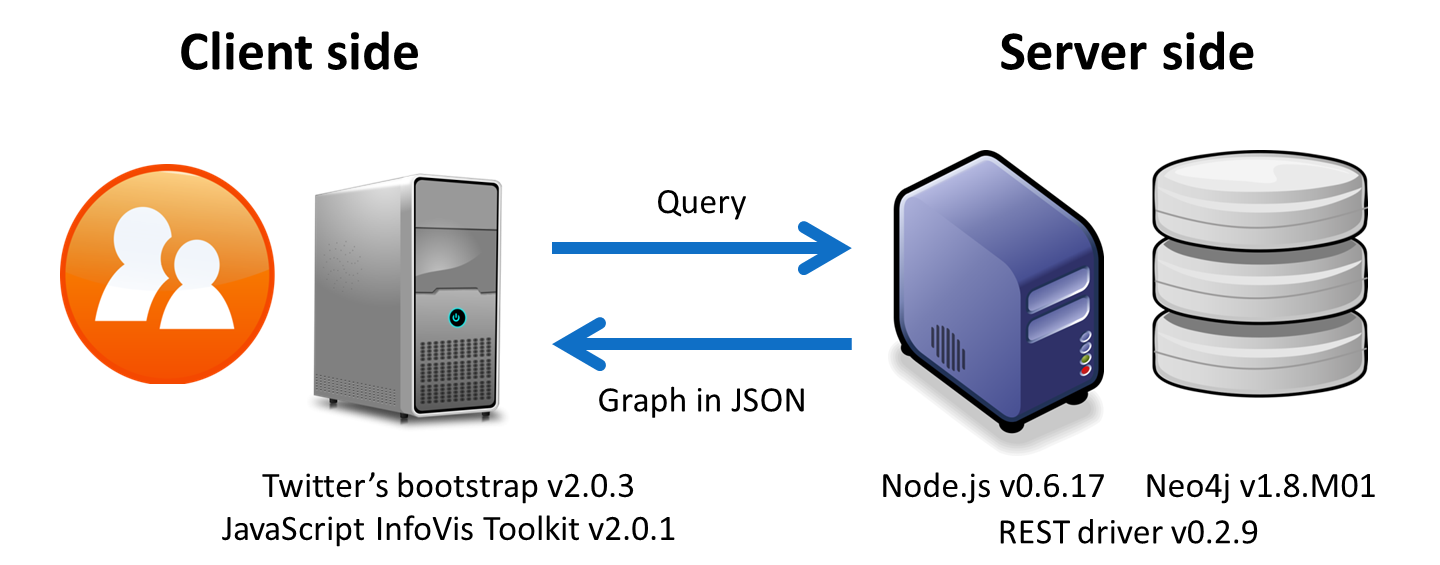
\includegraphics[width=\linewidth]{BlockDiagram.png}
\caption{ichem block diagram.}
\label{fig:BlockDiagram}
\end{figure*}

\subsection{Server Side}

On the server side, several packages were utilized (Figure \ref{fig:blockdiagram}). They all were the latest versions at the moment the experiments were carried out.

When I attempted to populate the entire 5,214,234 protein sequences into neo4j using node.js, an out-of-memory exception was thrown. Therefore, I wrote a script to extract 6,548 proteins that are from Homo sapiens (i.e. human). Likewise, I wrote a second script to extract 35,965 protein actions that link up any two of the 6,548 human proteins. The above filtering philosophy was also applied to the chemical side. I wrote a third script to extract 21,997 human protein-chemical links, a fourth script to extract 937 chemicals, and a fifth script to extract 16,204 chemical-chemical links.

However, the order to populate the above 5 kinds of data was apparently different from the order to extract them from the large files (Table \ref{tab:datasets}) because nodes must be created before relationships could be created. Therefore, I first populated 6,548 human proteins, followed by 35,965 human protein actions, followed by 937 chemicals, followed by 16,204 chemical-chemical links, followed by 21,997 human protein-chemical links. Finally I ended up with a neo4j graph of 7,486 nodes (including the root node) and 74,165 relationships of 5 relationship types (i.e. binding, ptmod, expression and activation for the 35,965 human protein actions, and interaction for the 16,204 chemical-chemical links and the 21,997 human protein-chemical links) with 2 node exact indexes, one for proteins and one for chemicals (Figure \ref{fig:BlockDiagram}). Figure \ref{fig:DataBrowser} shows the final graph in neo4j web administration.

\begin{figure*}
\centering
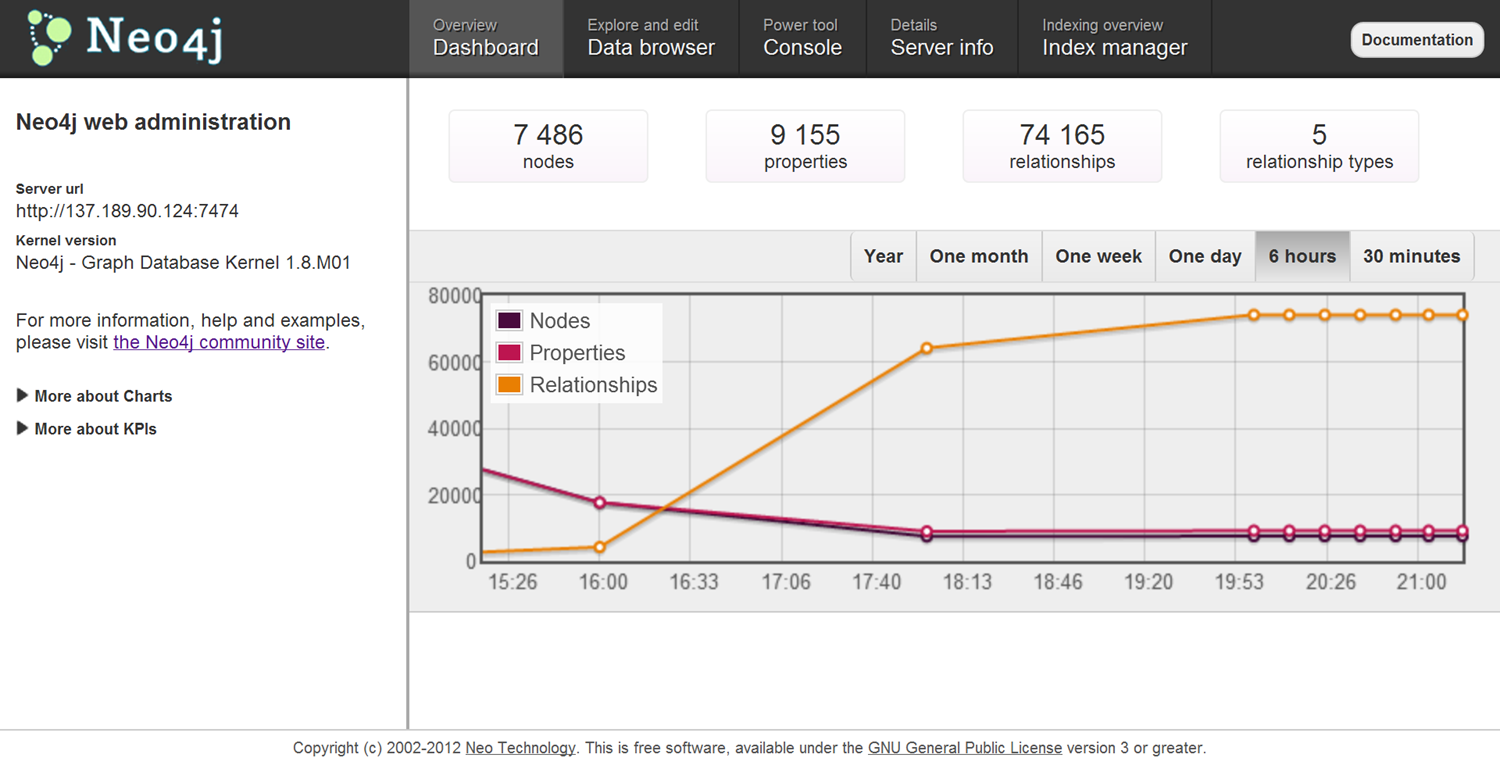
\includegraphics[width=\linewidth]{Dashboard.png}
\caption{Neo4j dashboard.}
\label{fig:Dashboard}
\end{figure*}

\begin{figure*}
\centering
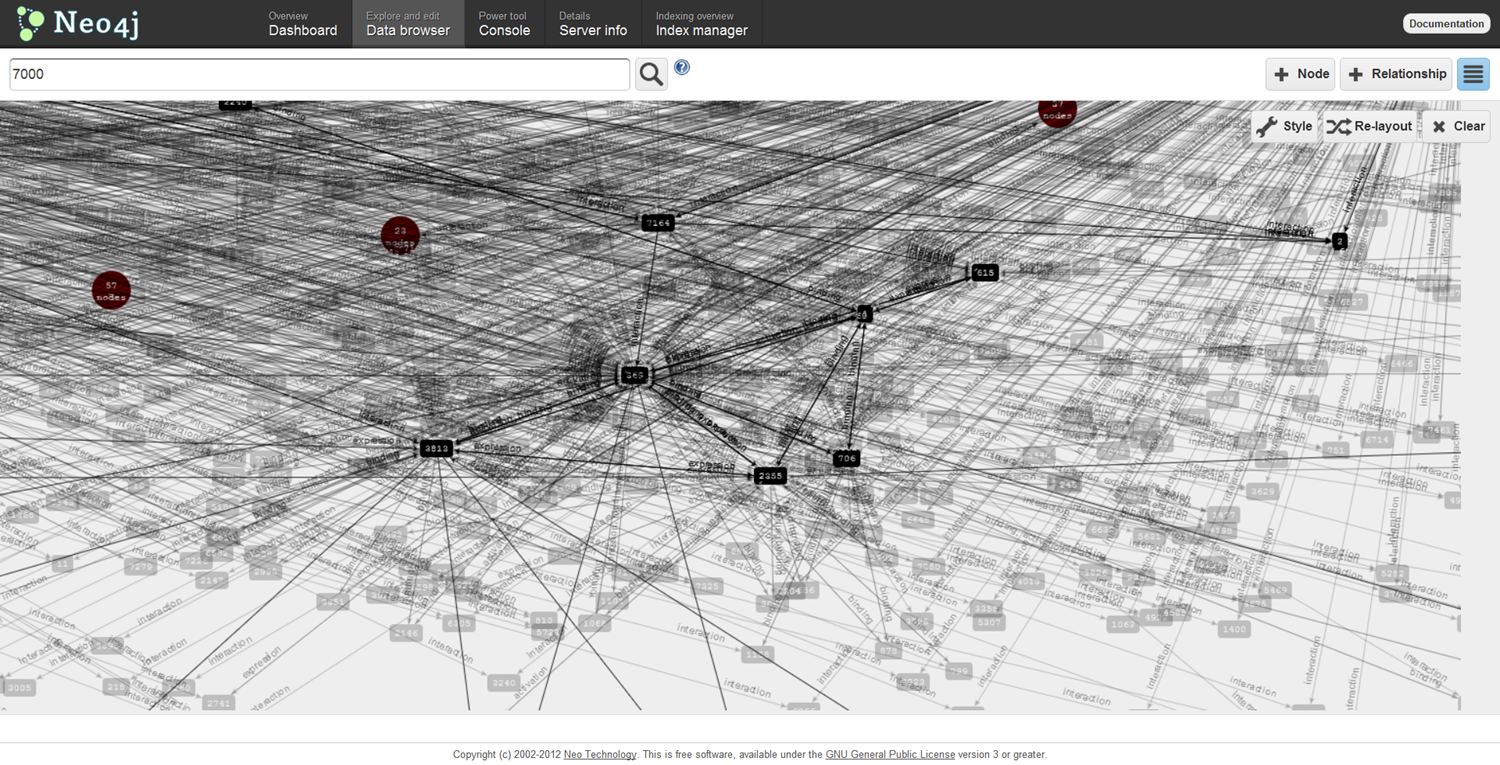
\includegraphics[width=\linewidth]{DataBrowser.png}
\caption{Neo4j data browser.}
\label{fig:DataBrowser}
\end{figure*}

I will provide several kinds of interaction queries, including but not limited to finding other chemicals which interact with the same protein given a chemical and finding other proteins which interact with the same chemical given a protein. These queries can easily be done in neo4j by graph traversal.

\subsection{Client Side}

On the client side, several packages were utilized (Figure \ref{fig:blockdiagram}). They all were the latest versions at the moment the experiments were carried out. I did a mini survey on about 20 graph visualization toolsuites, and eventually decided to settle down on JIT (JavaScript InfoVis Toolkit) for interactive data visualizations because it is free, open source, fully documented, and most importantly, powerful.

On the web client side, I will establish a web site with Twitter's bootstrap serving as a HTML5 and CSS3 template and jQuery serving as a javascript client for HTTP reqeusts and responses and graph visualization.

\begin{figure*}
\centering
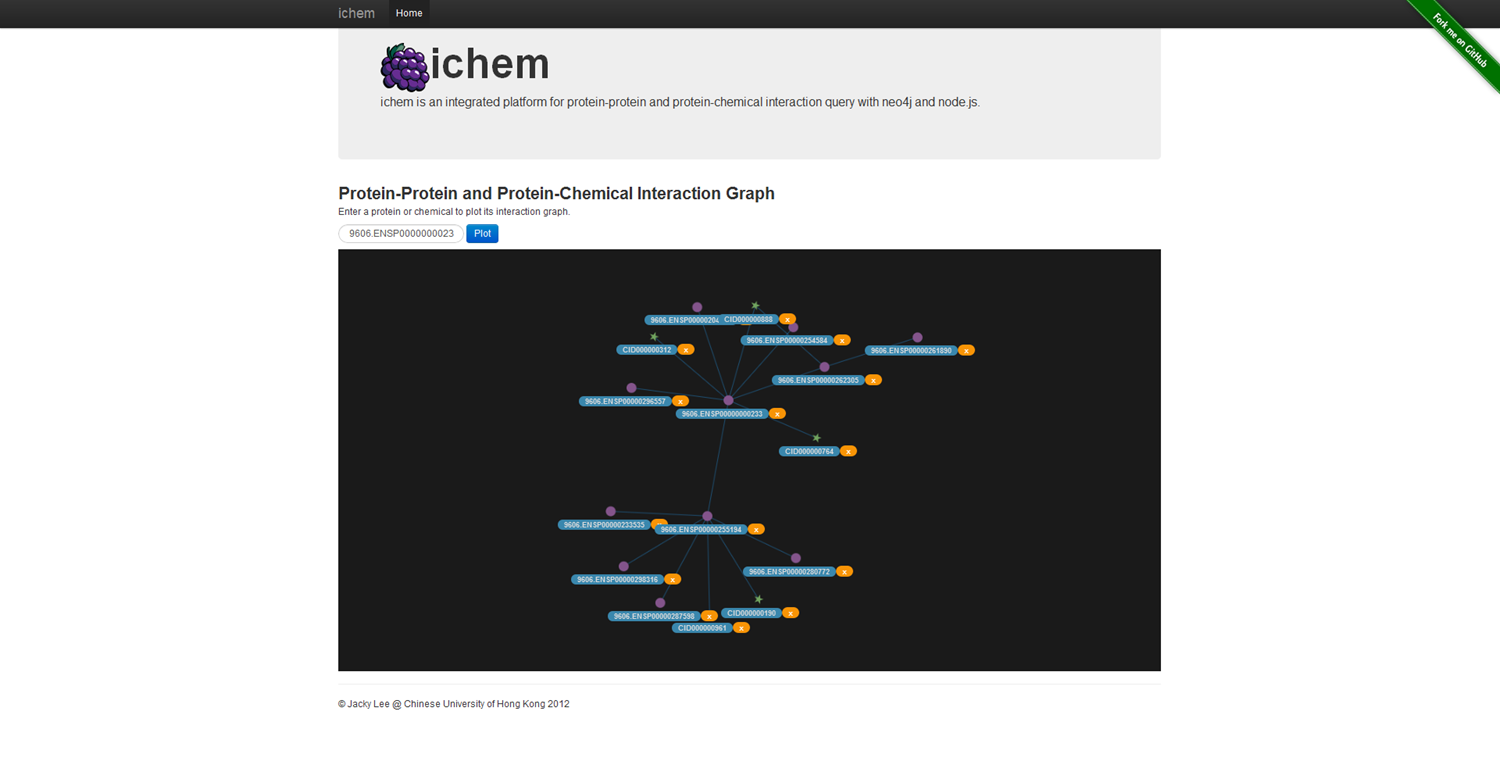
\includegraphics[width=\linewidth]{ichem.png}
\caption{ichem website.}
\label{fig:ichem}
\end{figure*}

\section{Availability}

ichem is free and open source under Apache License 2.0. It is available at https://GitHub.com/HongjianLi/ichem.

\section{Future Directions}

Incorporating the complete 23 GB STRING 9 and 22 GB STITCH 3 flat files into a neo4j graph database is definitely the first priority. Due to the huge data size, inserting records one by one no longer works. Instead, a bulk inserter in node.js should be implemented in advance in order to boost up the population procedure as well as to avoid out of memory exceptions.

Another possible way is to make use of fulltext indexing in neo4j. Generally speaking, a neo4j node index maps a key-value pair to a node. The mapping can be either exact or approximate, with the latter being known as fulltext indexing, implemented by the well-known Apache Lucene engine. It would be good to apply fulltext indexing to protein sequences and chemical names and aliases so that the input to search would no longer be limited to hard-to-memorize identities of proteins and chemicals.

\section{Conclusion}

I have integrated both protein-protein and protein-chemical interaction data utilizing neo4j and node.js, and established a modern website for fast query and vivid visualization. This project is novel in the sense that it is the first project to integrate both protein-protein and protein-chemical interaction data in a graphical way.

\bibliographystyle{unsrtnat}
\bibliography{../refworks}

\end{document}
